\chapter{Document Classification}

    In this chapter we introduce a problem of document (text) classification and commonly used approaches that are used to solve this problem.
    
    In this thesis we will improve upon one of the unsupervised approaches for this problem and add a supervised twist to it.

\section{Problem description and motivation} \label{sec:problem}

    Thanks to digitalizaion of books and texts, almost all human knowledge is now easily accessible to algorithms. 
    With rapid growth of social media platforms and electronic communication we see a new type of documents.
    These documents are not traditional books, but user generated content.
    Websites, blogs, facebook posts, tweets, G+ posts contain wast amounts of information that can be very valuable.
    Moreover, companies customer centers usually receive large amounts of questions and requests from customers that could be automatically processed.
    
    Automating text categorization and classification is therefore becoming increasingly important and fundamental task. 
    A major objective of text classification system is to semantically assignment one or more predefined categories to documents.
    
    Is this document a positive review? 
    Does this question asks about a person?
    Is this customer ticket related to software bug?
    All of the questions above are instances of a text classification problem.
    
    Usually, machine learning, statistical pattern recognition, or neural network approaches are used to construct classifiers automatically.
    This problem has significantly attracted attention from lots of researchers.

    \subsection{Sentiment analysis}
    
    \* % Cite something?
    
    One of the most popular instances of document classification is a sentiment analysis, \emph{SA}.
    SA is a process of determining whether a piece of writing is positive, negative or neutral.
    It is also known as opinion mining, deriving the opinion or attitude of a speaker. 
    A common use case for this technology is to discover how people feel about a particular topic.
    SA is widely applied to customer materials such as reviews or online and social media.
    It can answer questions like: ``Does this review suggests, that Eat\&Meet is a good place to eat (and meet)?'', ``Does the person likes his dog?''.
    
    There is a lot of ways how to approach document classification problem. 
    The most important thinks, that we consider about those approaches are accuracy and interpretability.
    Further we can consider also speed of required preprocessing, speed of actual classification, amount of required data and memory requirements. 
    
    In this thesis we revisit one of the older approaches called LSA and try to address some of its shortcomings.
    
    \* % popis aj ostatne datasety a veci ktore spominas: semantic relatedness, subjectivity/objectivity, question type, polarity

\section{Notation}

    In this section we provide a concise reference describing the notation and terms used in this thesis.
    
    \begin{table}[h]
        \centering
        \begin{tabular}{c l}
            $\circ$ & Hadamard product. \\
            $\alpha$ & Learning rate. \\
            $d_j$ & $j$-th document in our corpus.\\
            $D$ & Vocabulary. Denotes set (dictionary) of all used words in our dataset. \\
            $|D|$ & Size of the vocabulary. \\
            $E$ & Loss function such as L2.\\
            $N$ & Number of documents in the corpus. \\
            $n_w$ & Number of times word $w$ appears in the whole corpus. \\
            $Q$ & Cost function, very similar to loss function.\\
            $\Theta$ & Model parameters.\\
            $tf_{w,s}$ & Number of times word $w$ appears in sentence $s$. \\
            
        \end{tabular}
    \end{table}
    
    Our math notation is mostly influenced by programming practice.
    In this thesis we assume all vectors to be row vectors.
    We also assume natural broadcasting of some operations, like \circ for Hadamard product.
    
    Throughout this thesis we try to illustrate things with examples. 
    For consistency, we will use following sample corpus of sentences and labels:
    
    \begin{table}[h]
        \centering
        \begin{tabular}{c|c}
        \hline
            charlie is a good dog & 1 \\
            tiger is a bad cat & 0 \\
            oscar is a nice cat & 1 \\
            max is a bad dog & 0 \\
        \end{tabular}
        \caption{Example dataset}
        \label{tab:example:dataset}

    \end{table}
    
    This is an example "pet sentiment dataset". Labels denote, if the sentiment of the statement was positive ($1$) or not ($0$). 

    There are $|D|=11$ distinct words in the vocabulary $D$ of this corpus: 
    \begin{verbatim} a, bad, cat, charlie, dog, good, is, max, nice, oscar, tiger \end{verbatim}
    
    Later we will refer to them in this ordering, indexing from $1$. 
    Hence $D_4=\mathtt{charlie}$.


\section{Machine learning}
    
    Machine learning explores the study and construction of algorithms that can learn from and make predictions on data.
    More pragmatic description of machine learning is, that it is a magic process of fiddling with some numbers, until results look fine. \*% Cite usama.
    Being able to let algorithms automatically learn from data proved to be extremely important.
    Nowadays, almost any task can be improved or automatized thanks to such algorithms. 
    However, to use machine learning for some task, we usually need to specify the task in machine learning friendly way.    
    In this chapter, we introduce some of machine learning concepts in details.


    \subsection{Supervised machine learning}
    
    Supervised learning is a standard approach in machine learning. 
    Supervised algorithms learn to predict the best outputs for a given input.
    We denote the collection of input data, features, as $X$ and the corresponding expected outputs, labels, as $Y$.
    $X$ is usually a matrix of real values where rows of this matrix are individual samples.
    $Y$ is usually a vector of real values or integers. 
    Inside mathematical expression we usually denote labels as $y$,
    We refer to the pair of features and labels $(X, Y)$ as a dataset.
    In practice we usually have three such datasets: train, validation and test. 
    For the sake of this introduction we ignore this fact and we explain it in section \ref{sec:train:test:split}.
    
    In machine learning, we want to find a function $f$ such that for given sample $x_i$
    the functions output $\hat{y_i} = f(x_i)$ if very close to the the real label $y_i$.
    
    This is usually done by optimizing parameters $\Theta$ of a parametrized function $f_\Theta$,
    with regards to a loss function $E_y(\hat{y})$. 
    We refer to function $f_\theta$ as a \textit{model}.
    Common loss is an $L2$ loss function 
    $$E_y(\hat{y}) = \frac{1}{2}(y - \hat{y})^2 = \frac{1}{2}\sum_{i=1}^n (y_i - \hat{y_i})^2= \frac{1}{2}\sum_{i=1}^n (y_i - f_\Theta(x))^2$$  
    
    Formally we want to find parameter $\hat{\Theta}$ such that $\hat{\Theta} = argmin_\Theta \left(E_y(f_\Theta(x) \right)$. 
    This equation is usually not solved directly, but through an optimization process called learning \cite{Goodfellow-et-al-2016}. % deep learning book
    
    \subsubsection{Gradient descent}

    \textit{Gradient descent} method finds local minima of a usually multivariate function. 
    This is a well suited approach to use in context of supervised machine learning. 
    
    We use an observation, that if we follow the opposite direction of the gradient in a given point, 
    we arrive in a local minima. Example is on the picture \ref{obr:gradient}.
    
    In the context of machine learning, we optimize a cost function $Q$ of parameters $\Theta$, 
    $$Q(\Theta) = E_y(f_\Theta(x))$$
    
    We follow the opposite direction of gradient of the cost function $Q$ in respect to parameters $\Theta$. 
    We initialize $\Theta_0$ to small random numbers and we perform a gradient descent step
    
    $$\Theta^{t+1} = \Theta^t - \alpha \frac{\partial Q(\Theta^t)}{\partial \Theta^t} = \Theta^t - \alpha \nabla Q(\Theta^t)$$
    
    $\alpha$ denotes the size of the step we will make and is commonly known as a learning rate. 
    We perform the gradient descent step until we are not improving enough any more. 
    Formally we stop, when $|\Theta^{t+1} - \Theta^t| < \epsilon$ for a given $\epsilon$ \cite{bottou-bousquet-2008}.
    
    This process is also sometimes referred to as a batch gradient descent.

    \begin{figure}
    \centerline{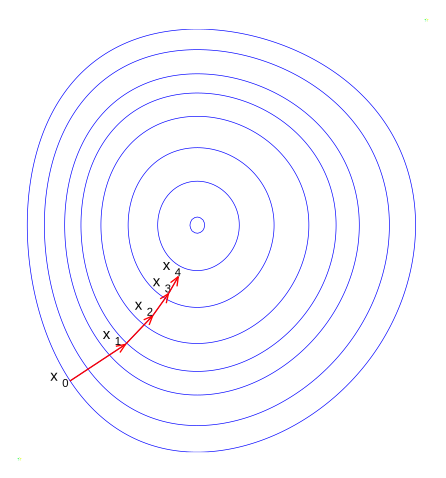
\includegraphics[width=0.4\textwidth]{images/gradient_descent}}
    \caption[Gradient descent]{Gradient descent \cite{pict}}
    \label{obr:gradient}
    \end{figure}
    
    \subsubsection{Stochastic gradient descent}
    
    During each gradient descent step, we need to evaluate the gradient of the loss function over the whole dataset.
    This is usually not feasible for larger datasets. 
    
    We can exploit that the cost function $Q$ can usually be rewritten as a sum of costs $Q_i$ for each data point $x_i$.
    
    $$Q(\Theta) = \sum_{i=1}^n Q_i(\Theta)$$
    
    $Q_i(\Theta)$ denotes the cost function computed on only the $i$-th element. 
    Instead of performing the gradient step on the whole $Q$, 
    we can perform a gradient step for each $Q_i$. 

    $$\Theta^{t+1} = \Theta^t - \alpha \frac{\partial Q_i(\Theta^t)}{\partial \Theta^t} = \Theta^t - \alpha \nabla Q_(\Theta^t)$$
    
    For appropriate $\alpha$ we usually see a much faster convergence than for gradient descent.
    
    \subsection{Feed forward neural network}
    There is a lot of ways how to construct function $f_\theta$ that we want to optimize. 
    One of the most popular ones is roughly inspired by the human brain and is called a \textit{feed forward neural network}. \* %citacia na Feed forward
    
    Neural network consists of small interconnected computational units (neurons) that are usually organized into a layers.
    Each unit takes some inputs, based on them produces an output and sends it to other units. 
    In a feed forward neural network, the signal is always moving forward,
    hence unit on the $k$-th layer can only take its input from previous layers \cite{Goodfellow-et-al-2016}.
    
    By adjusting the connections and theirs strengths, the network can learn to produce a specific output for a specific input.
    
    Simple neural network can be seen on an image \ref{obr:siet}.
    
    \begin{figure}[h]
    \centerline{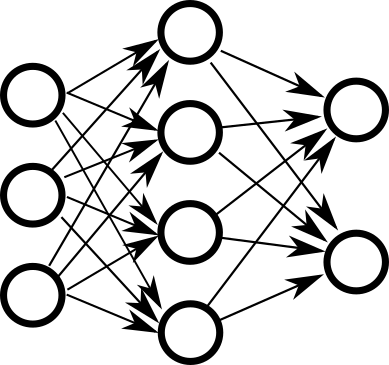
\includegraphics[width=0.4\textwidth]{images/neural_network}}
    \caption[Simple neural network with 2 layers, 3 inputs, 4 neurons and 2 outputs]{Simple neural network with 2 layers, 3 inputs, 4 neurons and 2 outputs}
    \label{obr:siet}
    \end{figure}
    
    The simplest realization of a unit is a weighted sum and application of activation function $g$. 
    Formally the unit receives a vector of inputs $x$ and computes output $g(\sum_{i=1}^n \theta_i x_i)$, 
    where $\theta_i$ is a connection strength to the $i$-th input.
    This one unit can be viewed as a simple one layer neural network with one output.
    
    Common realizations of function $g$ are: 
    \begin{itemize}
        \item logistic function $g(x) = \frac{1}{1+e^{-x}}$
        \item hyperbolic tangent $g(x)=\frac{e^x-e^{-x}}{e^x+e^{-x}}$
        \item relu $g(x) = \max(0,x)$ 
        \item leaky relu $g(x)=\log(1+\exp(x))$
    \end{itemize}
    
    One layer of such units can be compactly described thanks to matrix notation as
    $$y=g(X \Theta)$$
    
    $X$ represents the input matrix (number of samples $n$ times number of features $k$) and $\Theta$ is the matrix of weights (number of features $k$ times number of units $u$). Note that function $g$ is applied element-wise.
    
    One of the simplest classifiers and one of the simplest neural networks is the logistic regression.
    It is a one layer neural network with nonlinearity realized by the logistic (sigmoid) function $g(x) = \frac{1}{1+e^{-x}}$.
    This classifier has a few nice properties. 
    Derivation of its activation function can be very nicely expressed as $g'(x) = g(x)(1-g(x))$.
    Sigmoid outputs values in interval $[0,1]$ that can be directly viewed as a probability for given class.
    Because of these properties, the logistic regression is one of the most used classifiers and serves as a benchmark to great number of problems.
    
    
    The important observation about neural networks is, that we can chain such layers to form a deeper neural network.
    $$y=g_2(g_1(X \Theta_1) \Theta_2)$$
    
    $W_1$ are weight of hidden neurons (first layer) and $W_2$ are weight of output neurons (second layer). Note that $g_2$ (usually sigmoid) can be a different function than $g_1$ (usually relu).
    There is no consensus in the community about how to count the layers. 
    For example the simple network on picture \ref{obr:siet} could be seen as a $3$ layer neural network,
    because it has input units, hidden units and output units.
    In this thesis we will use the number of matrices $W$ that crates the model.
    
    In general, such multilayer feed forward neural networks represent very broad family of functions.
    They are in fact an universal approximator and can approximate any other function \cite{cybenko1989approximation}.
    However, we need to train them first.
    
    \subsubsection{Backpropagation} \label{sec:backprop}
    
    Backpropagation is a method for efficient computation of the gradient of a neural network.
    It relies on the the fact, that neural networks are just a simple compositions of matrix multiplications and function applications. 
    It also relies on the fact, that functions used in the units are differentiable (almost everywhere).
    
    \textit{Backpropagation} works in two parts, forward pass and backward pass.
    In the forward pass we feed to input to the network, compute activations of each layer and compute the final output.
    In the second pass, we make use of the chain rule and incrementally compute gradient with respect to each layer of the network.
    Then we use the gradient descent and optimize the parameters \cite{rumelhart1986david}.
    
    \* % write the equation
    
    
\section{Word and sentence representation}

    In order to apply machine learning techniques to a text classification, 
    we need to represent the text in a machine learning friendly way.
    Most machine learning algorithms expect the input in a form of vectors of numbers. 
    
    Because of this, we need a system to translate string sentences $s$ into vectors of numbers $e$.
    Such vector is usually called an embedding. 
    
    In  other words, we need to project words, sentences and documents into a vector space.
    We consider the sentences to be basically the same as documents. 
    They are just a sequence of words.
    
    \subsection{Local representation} \label{sec:local:representation}
    
    The simplest vector space is based on a local representation.
    In this representation, we use a vector space with $|D|$ dimensions, one for each word in the vocabulary.
    Value $v_i$ at the $i$-th position of the vector $v$ corresponds to a presence or an absence of the $i$-th words $D_i$ from the vocabulary $D$.
    Note, that $|D|$ in real applications easily exceeds $100\,000$ or even $1\,000\,000$.
    This may make this representation unusable for some applications (classification with SVM).
    
    One of the simplest local representations is a \textit{bag of words} (BOW) representation. 
    In this representation, values in vectors are binary, where $1$ means that the word was present in the text and $0$ means it was not.
    This can also be viewed as a simple one hot encoding.
    Optionally we can extend this to a term vector, where the number is not binary, but it express the real count of given word in the sentence.
    
    Let's look at our example corpus. 
    Our vector space would have $11$ dimensions and the first sentence would be represented as a vector
    $$e = (1, 0, 0, 1, 1, 1, 1, 0, 0, 0, 0)$$.
    
    This representation allows for simple sentence comparison. 
    Sentences $s_1$ and $s_2$ can be compared by comparing cosine similarity of their BOW embeddings $e_1$ and $e_2$.
    $$\mathrm{sim}(s_1, s_2) = \mathrm{sim}(e_1, e_2) = \frac{e_1 e_2}{||e_1||.||e_2||}$$
    For technical reasons we can also define a cosine distance. 
    $$\mathrm{dist}(s_1, s_2) = \mathrm{dist}(e_1, e_2) = 1- \mathrm{sim}(e_1, e_2) = 1 - \frac{e_1 e_2}{||e_1||.||e_2||}$$
    
    However this representation does not consider, that two words can be similar, even though they are not the same.
    For example words \texttt{nice} and \texttt{good} are considered to be completely different, even though they are not. 
    
    Second problem is, that this representation forgets the initial ordering of the words.
    We can address this problem, by using pairs of words instead of single words. 
    Pairs of words are called bigrams (n-grams).
    For example, the first sentence in our example dataset can be represented as bag of bigrams:
    
    $$e = ((4,7),(7,1),(1,6),(6,5))$$
    
    Third problem is, that this representation assigns the same weight to each word.
    The fact that two sentences both have a meaningless word \texttt{a} has the same effect on the similarity as if they both have semantically meaningful word \texttt{bad}. 
    This problem is partially solved by introducing term weights.
    
    
    \subsubsection{Term-weighting schemes} \label{sec:term:weights}
    
    To emphasize that some words in the corpus are more important than others we introduce a term-weighting schemes. 
    The idea is, that words like prepositions (\texttt{a}, \texttt{an}) and other words that are not very informative or redundant (\texttt{is}, \texttt{do}, \texttt{by}) should have smaller weights. 
    In practice, a list of \textit{stop words} is used to completely filter such words.
    
    Also words, that are to common in the dataset should have lower weights.
    If each sample is about a dog, we probably do not care about the word \texttt{dog}, because it is somehow redundant.
    
    However words, that appear multiple times in a sentence are probably important for this sentence and should have higher weights.
    
    Based on these two observations, a number of term-weighting schemes was proposed~\cite{salton1988term}.
    A term-weighting scheme assign a weight to a word $w$ in a sentence $s$ as term weight $t_{w,s}$.
    These weights usually consists of two parts, \emph{term frequency} and \emph{inverse document frequency}. 
    
    \emph{Term frequency} part $\mathrm{TF}_{w,s}$ reflects how important is word $w$ for sentence $s$.
    Common choices are:
    \begin{itemize}
        \item $\mathrm{sign}(\mathrm{tf}_{w,s})$, binary presence of the word in sentence. Also known as BOW.
        \item $\mathrm{tf}_{w,s}$, number of appearances.
        \item $\frac{\mathrm{tf}_{w,s}}{|s|}$, number of appearances normalized by length of the sentence.
        \item $1+\log(\mathrm{tf}_{w,s})$.
    \end{itemize}
    
    \emph{Inverse document frequency} part $\mathrm{IDF_w}$, reflects how important is the word $w$ for the whole corpus.
    Common choices are:
    \begin{itemize}
        \item $1$, unary.
        \item $\log \left(\frac{N}{n_w} \right)$, inverse document frequency.
        \item $\log \left( 1+\frac{N}{n_w} \right)$, smoothed inverse document frequency.
        \item $\log \left( \frac{max_{w'} n_{w'}}{n_w} \right)$, max inverse document frequency.
        \item $\log \left(\frac{N-n_w}{n_w} \right)$, probabilistic inverse document frequency.
    \end{itemize}

    Combination of such parts is called TF-IDF.
    Note, that these choices for $\mathrm{TF}_{w,s}$ and $\mathrm{IDF}_{w,s}$ are probabilistically grounded \cite{aizawa2003information}. %information perspective on TF-IDF
    
    Another popular weighting scheme that is usually used in document retrieval is $\mathrm{BM_{25}}$. 
    
    $$\mathrm{BM}_{25~w,s} = \log \left(\frac{N-n_w+0.5}{n_w + 0.5}\right)    \frac{\mathrm{tf}_{w,s} (1.2 + 1)}{\mathrm{tf}_{w,s} + 1.2  \left(1 - 0.75 + 0.75 \cdot \frac{N}{\text{avgdl}}\right)}$$
    
    This representation performs better than BOW and usually works the best for large documents in document retrieval \cite{li2014semantic}.
    
    Term weights can help to describe that different words, have different importance.
    However, they still cannot take into account, that two different words should have similar representation.
    
    
    \subsection{Distributed representation}
    
    To address the problem of high dimensionality and to allow different words to have high cosine similarity, we employ distributed representation.
    In this representation, dimensions do not correspond directly to words, but rather to some features of these words.
    In this representation the ''meaning`` of the word is split across multiple dimensions.
    We can view each dimension as if it holds some form of an abstract meaning \cite{le2014distributed}. 
    
    Simple but unrelated example of distributed representation is a binary representation of a number.
    
    To acquire a distributed representation, algorithms often make use of the distributional hypothesis.

    \subsubsection{Distributional hypothesis}
    
    Distributional hypothesis states, that words that appear in similar contexts tend to have similar meaning,
    even though they do not appear directly together \cite{harris1954distributional} \cite{Rubenstein:1965:CCS:365628.365657}. % distributional hypothesis 
    For example we can exchange words \texttt{dog} and \texttt{cat} in each sentence in our example corpus \ref{tab:example:dataset}
    and all sentences will still make sense. 
    The positive correlation between the words appearing in similar contexts and words having similar meaning was in fact empirically confirmed.
    
    Because of this, distributional hypothesis is used as a foundation for a lot of methods that try to capture the word semantic similarity \cite{rubenstein1965contextual}. 

    \subsection{Prediction based distributed representation}
    
    Number of researchers used neural networks to create a good, dense, distributed word representations \cite{pennington2014glove} \cite{DBLP:conf/icml/LeM14} \cite{rong2014word2vec}. % slovne vektory, some word2vec shit, glove word vectors
    These representations are also commonly called \emph{neural embeddings} or just word vectors.
    We will call these representations \emph{word vectors}.
    Word vectors proved to be very useful in broad range of natural language processing tasks. 
    
    Moreover, they manifest interesting algebraic properties. 
    
    $$v(king) - v(man) + v(woman) = v(queen)$$
    $$v(better) - v(good) + v(small) = v(smaller)$$
    
    $v$ denotes the word vector for given word.
    
    There are two main approaches for training word vectors with neural networks: skip-gram model and continuous bag of words model.
    Based on an embedding of an input word $x$, the \textit{skip-gram model} predicts words from the context of $x$ .
    On the other hand, the \textit{continuous bag of words model} tries to predict the word based on its context.
    
    These methods can be computationally intensive, and they require a lot of training data. 
    Moreover their training usually requires a lot of well chosen hyper-parameters and tricks \cite{DBLP:journals/corr/MikolovSCCD13} \cite{vajdova2017}. % podvzorkovanie
    

    \subsection{Count based distributed representation}
    
    Count based methods create co-occurrence matrix and try to extract its underlying structure.
    These approaches are very popular before the raise of neural networks and neural embeddings.
    
    There is multiple ways how to extract some structure out of the Co-occurrence matrix.
    For example, latent Dirichlet allocation (LDA) \ref{blei2003latent} constructs a probabilistic model of each document. 
    It assumes, that each document is created as a mixture of topics and that each topic is just a distribution over words. 
    
    Second popular class of approaches relies on performing some matrix factorization on the co-occurrence matrix.
    In this thesis we build on of these factorization approaches.
    
    \subsubsection{Latent semantic analysis} \label{sec:lsa}
    
    For the purposes of this thesis we consider the \emph{latent semantic indexing} (LSI) to be the same as \emph{latent semantic analysis} (LSA) \cite{deerwester1990indexing}.
    For simplicity, we will refer only to the LSA.
    
    \emph{Latent semantic analysis} is one of the standard approaches to identify hidden variables describing the data.
    In the context of natural language classification it extracts and infers relations of expected contextual usage of words in documents.
    It does so without any humanly constructed dictionaries, knowledge bases, semantic networks, grammars or syntactic parsers.
    
    This property proves to be extremely useful and is not specific only to the LSA.
    Machine learning algorithms that rely only on data $X$ and do not need any form of labels $Y$ are commonly called unsupervised.
    The problem is, that data is usually very easy to acquire (just set of some documents), but labels $Y$ are very hard and costly, because they may require human annotation.
    
    LSA starts with a co-occurrence matrix $M'$. 
    Each cell $M'_{i,j}$ of this matrix contains number representing the frequency with which  the  word $D_i$ appears in the document $d_j$.
    Afterwards each cell entry is weighted by a function that expresses both the words importance in the particular document and the word importance in the general corpus.
    A weighting scheme such as TF-IDF can be used.
    We denote the reweighted matrix $M$. 
    
    Next, LSA applies singular value decomposition (SVD) to the matrix.
    In principle, SVD achieves a two-mode factor analysis and positions both terms and documents in a single space defined over the extracted dimensions.
    In case a different matrix factorization is used such as non negative matrix factorization, we would arrive to probabilistic latent semantic analysis.
    
    SVD breaks down the document matrix $M$ into three matrices $U$, $\Sigma$, $V$,\cite{papadimitriou2000latent} % interpretation of lsa, steal some introduction 
     % first lsi/lsa?
    \cite{maas2011learning} % lda, vector space model
    \cite{wiemer2004latent} % Latent semantic analysis
    \cite{landauer1998introduction} % introduction to lsa 
    such that $$M=U \Sigma V^T$$ 

    $U$ and $V$ are orthogonal matrices and $\Sigma$ is a diagonal matrix.
    
    {$$
\begin{matrix} 
 M &  ~~ U & \Sigma & V^T \\
 \textbf{d}_i^T &  & &  \\
 \downarrow &  & &  \\
\begin{bmatrix}
x_{1,1} \dots  x_{1,N} \\
\vdots ~~~  \ddots ~~~ \vdots \\
x_{j,1} \dots  x_{j,N} \\
\vdots ~~~ \ddots ~~~ \vdots \\
x_{|D|,1} \dots  x_{|D|,N} \\
\end{bmatrix}
=
&
\textbf{u}_j \rightarrow
\begin{bmatrix} 
\begin{bmatrix} & \textbf{u}_1 & \end{bmatrix} \\
\vdots \\
\begin{bmatrix} & \textbf{u}_{|D|} & \end{bmatrix}
\end{bmatrix}
&
\cdot
\begin{bmatrix} 
\sigma_1 \dots ~~~ 0 \\
\vdots ~~~ \ddots  \vdots \\
0  \dots  \sigma_k \\
\end{bmatrix}
&
\cdot
\begin{bmatrix} 
\begin{bmatrix} \, \\ \, \\ \textbf{v}_1^T \\ \, \\ \,\end{bmatrix} 
\dots
\begin{bmatrix} \, \\ \, \\ \textbf{v}_N^T \\ \, \\ \, \end{bmatrix}
\end{bmatrix}
\end{matrix}
$$}

    $U$ describes the original row entities (words) as vectors of derived orthogonal  factor values. 
    $V$ describes the original column entities (documents) in the same way.
    $\Sigma$ containing scaling values such that when the three components are matrix multiplied, the original matrix is reconstructed.

    It was shown that any matrix can be decomposed perfectly in a such way, using no more factors than the smallest dimension of the original matrix.
    
    Moreover we can construct an approximation with reduced rank by setting all but the $k$ biggest entries in $\Sigma$ to zero. 
    This effectively reduces the number of columns of $U$ to $k$ and similarly number of rows of $V^T$.
    The thesis behind LSI is that those less important dimensions correspond to “noise” due to word-choice variability.
    
    Note that due to this reduction we inevitably loose some of the information. 
    We can see this as forgetting some of the less often words.

    An interesting property of SVD is that the generated approximation is the closest matrix of its rank to the original in the least-squares sense \cite{berry1995using}.

    In practice, computing the full SVD decomposition would be time and memory demanding and even unfeasible.
    Because of that, we directly compute the lower rank approximation with $k$ dimensions,
    such that $M \simeq U_k \Sigma V_k^T$ \cite{halko2011finding}. %fast svd
    Moreover, we do not even need to have access to the full matrix $M$ and we can compute the decomposition in an incremental manner \cite{brand2006fast}. % incremental svd
    
    Not only we can incrementally adjust the decomposition when adding a new document into the corpus, we can remove a document as well.
    Incremental SVD could in theory be used in the stochastic gradient descent setting.
    
    From now on, we drop the subscript $k$ and matrices $U$, $\Sigma$ and $V$ in the later text are assumed to have only $k$ dimensions.
    
    
    \subsubsection{LSA for document classification}
    
    In context of document classification, we first construct our vocabulary $D$ from our training data. 
    We can filter out words that we know, are not relevant, or that have only a few appearances in the corpus.
    
    Now we can transform sentences into their BOW representations.
    Afterwards, we compute all necessary statistics required by our chosen weighting scheme.
    In case of TF-IDF, we compute the number of appearances of each word in our text $n_w$. 
    This can be done efficiently by making use of fast matrix operations and libraries implementing linear algebra.
    Having these statistics, we can reweigh all words with them and construct the term matrix $M$.
    
    Then we factorize $M$ an compute the matrices $U$, $\Sigma$, $V$. 
    In theory, we could directly read the document embeddings $v$ from the matrix $V$.
    For practical purposes, the matrix $V_k$ is usually not stored and sometimes not even computed. 
    
    To compute the embedding, we take the document term vector $d_i$ and employ a relationship $$d_i^T = U \Sigma v_i^T$$
    
    Because $U$ is orthogonal and $\Sigma$ is diagonal, we get
    
    $$\Sigma^{-1} U^T d_i^T = v_i^T $$

    $$v_i = d_i U \Sigma^{-1} $$
    
    Note, that $\Sigma^{-1}$ is easy to compute, because $\Sigma$ is a diagonal. 
    We just need to invert each number on the diagonal.  
    
    As was experimentally shown in my bachelor thesis \cite{macko2016} 
    and by other researchers \cite{levy2015improving}, $\Sigma$ may not reflect the importance of each feature very well.
    
    Because of that, a simpler relationship is usually employed
    
    $$v_i = d_i U $$
    
    This process can have a different interpretation.
    Each entry in matrix $U$ is the distributed representation for one word.
    The matrix multiplication selects words, that are present in the document and computes a weighted sum of them.
    
    Important part is, that we can compute such embedding even for unseen documents.
    The problem is, that we have to filter all words that are not present in $D$. 
    However, because this method is fully unsupervised, we can make use of any unlabeled data (documents, that do no have known label). 
    Factorized matrix $M$ can contain documents, that we do not have the label for.
    
    Finally, we perform the classification.
    Matrix of embeddings $v_i$ are considered to be the document features and are used as an input $X$ to some classifier. 
    A popular choices for classifier are a SVM or neural networks.
    First we train the classifier on some training set of documents and ther labels.
    Then we can easily predict labels for unseen documents.
    
    We can break down the whole process into three parts: weighting, decomposition and classification.
    We denote the weighting part as $W$, the decomposition part as $S$ (SVD) and the classification part as $C$.
    
    \subsubsection{LSA pitfalls}

    Even though LSA was shown to perform well in document retrieval applications and it can capture some basic semantic properties of words,
    it has certain limitations when applied to classification tasks. 
    
    The problem is, that LSA does not incorporate the information about document classes. 
    It finds the most representative features and not the most discriminative ones \cite{berry1995using}.
    In other words, it finds embedding that is the best for reconstructing the documents.
    Because of that, infrequent words that have high discriminatory power (are important for the task), may be filtered out.
    
    For example, LSA computed on our example corpus \ref{tab:example:dataset} would focus on capturing the words \texttt{a}, \texttt{is}, \texttt{dog} and \texttt{cat},
    event though they are completely irrelevant to our prediction task.
    
    \subsection{Relationship of prediction and count based representations}
        
    LSA and other count based techniques used to be very popular alternative to local representations.
    However after the raise of neural networks, they were soon overshadowed by neural word embeddings.
    
    Prediction based models achieved much better performance across multiple word relatedness tasks, categorization tasks, synonym tasks and analogy tasks \cite{baroni2014don}. % do not count, predict
    
    During these evaluations, they obtained the word representations by training on a big monolingual dataset, like wikipedia.
    Then they used a prepared pairs of related words (synonyms or words from the same category) and tested,
    how similar are the vector representations of related words. 
    They measured how well the word vector similarity correlates with the actual relatedness. 
    Count based methods achieved Pearson correlation coefficient $0.74$ and were outperformed by prediction based methods which achieved $0.84$ \cite{baroni2014don}.
    
    This and the hype around neural networks led to recent extreme popularity of prediction based embeddings,
    even though they were much less understood and less ''mathematically grounded``.
    
    Later it was shown, that these two approaches are in fact very similar.
    It was proven, that a prediction based model skip-gram with negative-sampling (SGNS) 
    is implicitly factorizing a word-context matrix $M$,
    whose cells are the point-wise mutual information (PMI) of the respective word and context pairs, 
    shifted by a global constant~\cite{levy2014neural}. % word2vec as matrix factorization 
    
    These results suggest, that these two approaches are somehow equivalent and with proper weights the LSA should achieve similar results as skip-gram model. 
    However in practice, this was not the case.
    
    Prediction based models require a lot of hyperparameters, that cannot be learned and need to be set up manually,
    or through excessive search.
    On the other hand, count based models usually do not require a lot of parameters, besides the number of dimensions of the resulting embedding. 
    
    Levy et al. \cite{levy2015improving} % word2vec hacks in lsi
    showed, that much  of  the  performance  gains  of  neural embeddings  are  due  to such hyperparameters and certain system design choices, rather than the embedding algorithms themselves. 
    Furthermore they showed that traditional (count based) distributional models
    can also benefit from such hyperparameters and design choices.
    
    After incorporating these insights into the count based methods, 
    they observed mostly local or insignificant performance differences between quality of count based embeddings and prediction based embeddings.
    
    Note, that these experiments were done on a large bodies of text like English Wikipedia.   
    On small datasets it was empirically shown, that count based methods actually outperform the neural networks.\cite{altszyler2016comparative}. % lsa vs word2vec on samall corpora
    
    
